
\documentclass[12pt, addpoints]{exam}
\usepackage[utf8]{inputenc}
\usepackage[portuguese]{babel}
\usepackage{multicol}
\usepackage{graphicx}
\usepackage{amsmath}
\usepackage{xcolor}
\usepackage[a4paper, portrait, margin=2cm]{geometry}

\setlength{\columnsep}{1cm}

        \begin{document}

        \begin{minipage}[l]{0.75\linewidth}
            \begin{flushleft}
                {\bf \Large Prova bimestral - LQ2N (2B)}
            \end{flushleft}
        \end{minipage}
        \begin{minipage}[r]{0.20\linewidth}
            \begin{flushright}
                {\bf \Large Código: 0}
            \end{flushright}
        \end{minipage}
        \vspace{0.5cm} \hrule \vspace{0.5cm}
        \begin{minipage}{0.75\linewidth}
            Aluno:
        \end{minipage}
        \begin{minipage}{0.20\linewidth}
            Data: 31/10/2022
        \end{minipage}
        \vspace{0.5cm} \hrule \vspace{0.5cm}

        \begin{center}
\textcolor{red}{\emph\Large Correction version}\end{center}
\begin{questions}
\begin{multicols*}{2}
\question[33] Considere uma partícula de massa    6.53 kg e velocidade    8.76 m/s. Determine a sua energia cinética.

\begin{center}
\begin{minipage}[c]{0.75\linewidth}
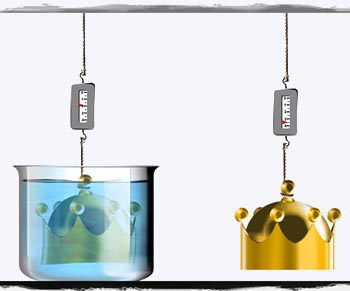
\includegraphics[width=\textwidth]{MWE001.jpg}
\end{minipage}

\end{center}
\begin{oneparchoices}
\choice 638.96 J\choice 578.22 J\choice 25.13 J\choice 17.48 J\choice 250.58 J\choice 221.1 J\choice 55.17 J\choice 39.7 J\choice 25.03 J\choice 4.85 J\end{oneparchoices}

\begin{oneparchoices}
\choice 0.0\choice 0.0\choice 0.0\choice 0.0\choice 33\choice 0.0\choice 0.0\choice 0.0\choice 0.0\choice 0.0\end{oneparchoices}
\question[23] Durante sua trajetória uma partícula realizou um trabalho de   -8.89 J. Qual foi a variação da sua energia cinética?

\begin{oneparchoices}
\choice -8.89 J\choice -8.76 J\choice 4.96 J\choice -9.63 J\choice -2.27 J\choice -1.28 J\choice 8.97 J\choice -0.64 J\choice -9.46 J\choice -7.22 J\end{oneparchoices}

\begin{oneparchoices}
\choice 23\choice 0.0\choice 0.0\choice 0.0\choice 0.0\choice 0.0\choice 0.0\choice 0.0\choice 0.0\choice 0.0\end{oneparchoices}
\end{multicols*}
\end{questions}
\newpage
        \begin{minipage}[l]{0.75\linewidth}
            \begin{flushleft}
                {\bf \Large Prova bimestral - LQ2N (2B)}
            \end{flushleft}
        \end{minipage}
        \begin{minipage}[r]{0.20\linewidth}
            \begin{flushright}
                {\bf \Large Código: 1}
            \end{flushright}
        \end{minipage}
        \vspace{0.5cm} \hrule \vspace{0.5cm}
        \begin{minipage}{0.75\linewidth}
            Aluno:
        \end{minipage}
        \begin{minipage}{0.20\linewidth}
            Data: 31/10/2022
        \end{minipage}
        \vspace{0.5cm} \hrule \vspace{0.5cm}

        \begin{center}
\textcolor{red}{\emph\Large Correction version}\end{center}
\begin{questions}
\begin{multicols*}{2}
\question[33] Considere uma partícula de massa    7.97 kg e velocidade    1.84 m/s. Determine a sua energia cinética.

\begin{center}
\begin{minipage}[c]{0.75\linewidth}
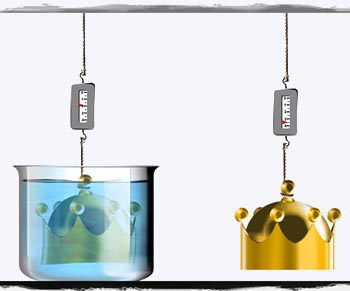
\includegraphics[width=\textwidth]{MWE001.jpg}
\end{minipage}

\end{center}
\begin{oneparchoices}
\choice 5.17 J\choice 100.21 J\choice 13.49 J\choice 200.95 J\choice 25.25 J\choice 31.64 J\choice 756.72 J\choice 250.71 J\choice 819.85 J\choice 453.43 J\end{oneparchoices}

\begin{oneparchoices}
\choice 0.0\choice 0.0\choice 33\choice 0.0\choice 0.0\choice 0.0\choice 0.0\choice 0.0\choice 0.0\choice 0.0\end{oneparchoices}
\question[23] Durante sua trajetória uma partícula realizou um trabalho de   -0.99 J. Qual foi a variação da sua energia cinética?

\begin{oneparchoices}
\choice 3.08 J\choice 6.13 J\choice 7.68 J\choice 1.2 J\choice -8.92 J\choice 9.77 J\choice -0.99 J\choice 9.22 J\choice -9.91 J\choice -4.78 J\end{oneparchoices}

\begin{oneparchoices}
\choice 0.0\choice 0.0\choice 0.0\choice 0.0\choice 0.0\choice 0.0\choice 23\choice 0.0\choice 0.0\choice 0.0\end{oneparchoices}
\end{multicols*}
\end{questions}
\newpage\end{document}